\chapter{METODOLOGI}
\section{Metode Penelitian}
\hspace{25pt} Penelitian ini dilakukan dengan 2 metode yaitu metode penginderaan jauh dan gravitasi. Data yang diolah merupakan data sekunder dimana untuk metode penginderaan jauh menggunakan data Landsat 8 yang diperoleh dari \href{https://earthexplorer.usgs.gov/}{\textit{EarthExplorer}} serta data \textit{gravity} yang diperoleh dari \href{https://ddfe.curtin.edu.au/models/GGMplus/}{GGMPlus}. Metode penginderaan jauh digunakan untuk pemetaan sebaran potensi panas bumi ditinjau dari nilai NDVI, LST dan FFD sedangkan metode gravitasi digunakan untuk pemodelan bawah permukaan dan untuk menemukan sesar menggunakan analisis derivatif. Penelitian dilakukan di daerah Tiris - Gunung Lamongan dengan koordinat 7.941955°-8.005723°LS dan 113.325397°-113.402531°BT.

\section{Data dan Perangkat Lunak}
\hspace{25pt} Beberapa data dan perangkat lunak \textit{(software)} yang digunakan untuk pengolahan data pada penelitian ini yaitu:
\begin{enumerate}
	\item Peta geologi Gunung Lamongan, diperoleh dari \textit{website} Pusat Vulkanologi dan Mitigasi Bencana Geologi
	\item Data Landsat 8 (Landsat Collection 2 Level-2), diperoleh dari \href{https://earthexplorer.usgs.gov/}{https://earthexplorer.usgs.gov/}, merupakan data utama metode penginderaan jauh. Data yang digunakan hanya band 4,5 dan 10. Pengolahan dilakukan untuk memeperoleh NDVI dan LST.\sloppy

	\item DEMNAS, diperoleh dari \href{https://tanahair.indonesia.go.id/demnas}{https://tanahair.indonesia.go.id/demnas}, merupakan data elevasi untuk memeperoleh kelurusan yang selanjutnya untuk analisis FFD.
	
	\item Data gravity, diperoleh dari \href{https://ddfe.curtin.edu.au/models/GGMplus/}{https://ddfe.curtin.edu.au/models/GGMplus/}, merupakan data gravity dan hanya diambil data \textit{gravity disturbance}, geoid, dan dem. Sesuai dengan daerah penelitian, maka file GGMplus yang dipilih memiliki koordinat S10E110.
	
	\item Matlab, digunakan untuk ekstraksi data gravity dari GGMplus terkhusus pada daerah penelitian sehingga tidak semua data pada koordinat S10E110 digunakan.
	
	\item Google Earth, digunakan untuk memberi tanda pada daerah penelitian yang selanjutnya digunakan untuk pembuatan \textit{shapefile} pada ArcMap
	\item ArcMap 10.8, digunakan untuk membuat \textit{shapefile} pada daerah penelitian, memotong data Landsat, dan pengolahan LST.
	\item Geomatica, digunakan untuk konversi data DEM ke hillshade untuk analisis FFD
	\item Microsoft Excel, digunakan untuk perhitungan koreksi metode gravitasi, analisis derivatif FHD dan SVD.
	\item Global Mapper 23.1, digunakan untuk pembuatan \textit{grid} lokal dan regional untuk \textit{terrain correction}
	\item Oasis Montaj, digunakan untuk konversi latitude/longitude ke UTM, perhitungan \textit{terrain correction}, \textit{grid} dan \textit{layout} peta Complete Bouguer Anomaly (CBA), pemisahan anomali lokal dan regional.
	\item Grav2DC, digunakan untuk pemodelan bawah permukaan
	\item TexStudio, digunakan untuk pengetikan tugas akhir.
\end{enumerate}
\section{Alur Kerja Penelitian}
Alur kerja penelitian ini secara umum ditunjukkan oleh diagram alir pada Gambar \ref{fig:FlowChart}. Secara lebih rinci alur kerja penelitian adalah sebagai berikut
\begin{enumerate}
	\item Studi Literatur \\
	Sebelum melakukan penelitian dilakukan studi literatur terkait prinsip metode penginderaan jauh khususnya untuk data Landsat 8 serta metode gravitasi. Kemudian dilakukan juga studi literatur tentang sumber panas bumi khususnya di Jawa Timur sebelum akhirnya ditetapkan daerah Tiris-G.Lamongan sebagai lokasi penelitian. Sumber bacaan yang digunakan seperti buku, jurnal, artikel ilmiah, tugas akhir dan tesis terdahulu. Selain itu, dilakukan juga studi tentang penggunaan software untuk pengolahan data.
	\vskip 5pt
	\begin{figure}
		\centering
		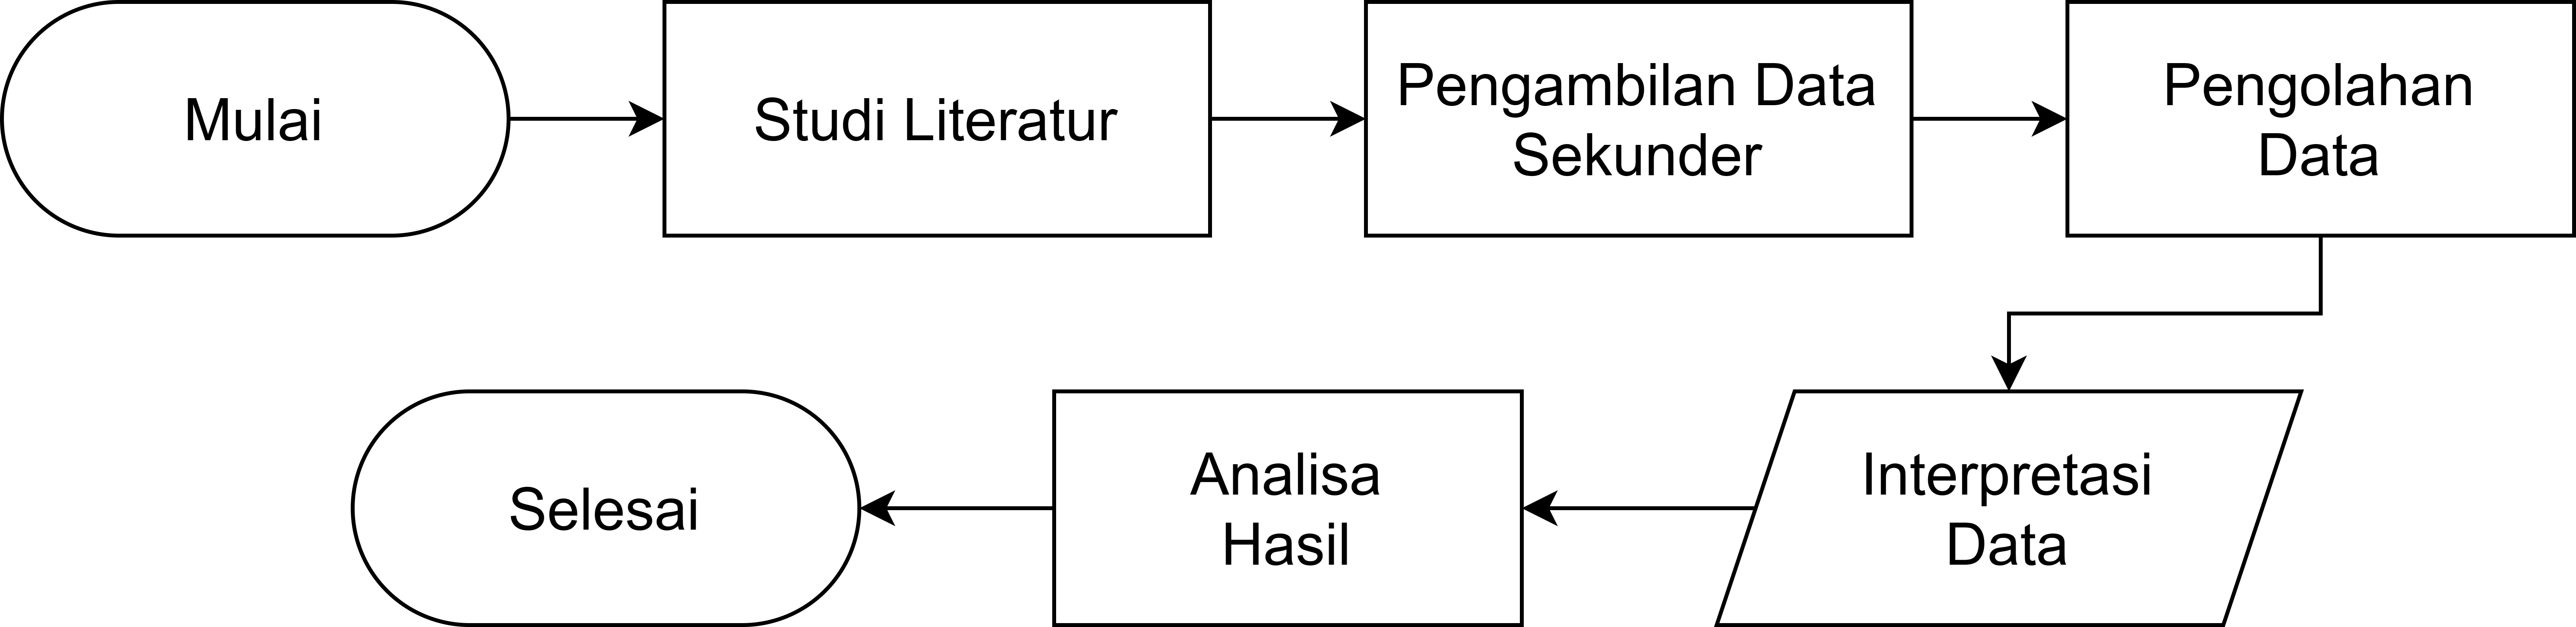
\includegraphics{Figs/FC.png}
		\caption{Alur Kerja Penelitian}
		\label{fig:FlowChart}
	\end{figure}

	\item Pengambilan Data Sekunder\\
	Data yang digunakan adalah data sekunder dimana untuk metode penginderaan jauh menggunakan data Landsat 8 dan DEMNAS. Kemudian untuk metode gravitasi digunakan data dari GGMplus. Untuk data Landsat 8 diperoleh dari \href{earthexplorer.usgs.gov }{earthexplorer.usgs.gov } dengan memilih daerah penelitian dengan tutupan awan paling minimum untuk hasil penelitian yang lebih baik sedangkan untuk data DEMNAS diperoleh dari \href{tanahair.indonesia.go.id/demnas}{tanahair.indonesia.go.id/demnas} . Kemudian, data gravitasi diperoleh dari GGMplus melalui \href{ddfe.curtin.edu.au/models/GGMplus/}{ddfe.curtin.edu.au/models/GGMplus/}. GGMplus menyajikan data dalam potongan potongan setiap 5x5 sehingga data yang dipilih adalah data dengan koordinat S10E110 dimana mencakup daerah penelitian. Terdapat beberap data yang disajikan GGMplus, data yang diambil adalah gravity disturbances dimana data ini telah terkoreksi tidal, drift dan lintang. Kemudian juga diambil data geoid untuk melakukan free air correction dan terkahir adalah data DEM untuk mengetahui elevasi setiap data pada gravity disturbances.
	\vskip 5pt
	\item Pengolahan Data Landsat dan DEMNAS\\
	Data Landsat digunakan untuk memetakan sebaran panas bumi. Hal ini dapat diketahui melalui nilai land surface temperature (LST).  Untuk mendapatkan nilai LST ini dilakukan tahapan-tahapan seperti pada sub-bab 2.4.3. Perhitungan-perhitungan tersebut dilakukan menggunakan fitur raster calculator pada ArcMap. Sebelum itu data dan Landsat dan DEMNAS masih berupa cakupan willayah yang lebih luas sehingga perlu dilakukan pemotongan. Pemotongan ini dimulai dengan membuat shapefile pada daerah penelitian dengan memberi pinpoint atau polygon pada Google Earth. Kemudian file dari Google Earth ini yang berformat kmz dibuka ke ArcMap untuk dikonversi ke format layer dan kemudian dilanjutkan pembuatan shapefile. Hal ini dilakukan agar tidak perlu melakukan georeferencing ulang pada daerah penelitian terhadap data Landsat. Selanjutnya shapefile yang telah diperoleh dilakukan extract to mask pada data Landsat dan DEMNAS. Data Landsat akhirnya dapat dilakukan perhitungan menggunakan raster calculator sedangkan untuk data DEMNAS dilakukan pengolahan pada software Geomatica untuk memperoleh kelurusan dengan mengonversinya kedalam hillshade. Kemudian dapat dilakukan analisis fault fracture density (FFD) pada ArcMap. Hasil akhir dari pengolahan ini adalah peta NDVI, LST dan FFD.
	\vskip 5pt
	\item Pengolahan Data Gravity \\
	Data gravity disturbances yang diperoleh dari GGMplus telah terkoreksi tidal, drift dan lintang sehingga tahapan berikutnya adalah melakukan koreksi mulai dari free air correction, terrain correction, Bouguer correction dan akhirnya diperoleh peta complete Bouguer anomaly. Koreksi free air correction dilakukan pada Microsoft Excel dan untuk terrain correction tidak dilakukan menggunakan hammer chart tetapi menggunakan Oasis Montaj. Terrain correction menggunakan Oasis Montaj membutuhkan data DEM dalam grid dari lokasi penelitian dengan koreksi lokal dan regional. File grid tersebut diperoleh menggunakan Global Mapper dimana untuk koreksi lokal daerah penelitian diperluas 1000 UTM dan untuk regional diperluas 10000 UTM pada masing-masing koordinat bujur dan lintang. Selanjutnya adalah koreksi Bouguer dimana koreksi ini membutuhkan nilai densitas batuan bawah permukaan. Nilai ini menggunakan metode Parasnis seperti yang ditunjukkan pada persamaan \ref{eqn:Parasnis}. Kemudian dapat diperoleh peta complete Bouguer anomaly melalui persamaan \ref{eqn:CBA2}.  Peta CBA yang telah diperoleh kemudian dilakukan pemisahan anomali menggunakan Oasis Montaj. Filter yang digunakan adalah butterworth filter. Kemudian setelah diperoleh peta anomali residual, dilakukan pemodelan bawah permukaan menggunakan Grav2DC dan analisis derivatif FHD dan SVD menggunakan Excel.
	\vskip 5pt
	\item Interpretasi Data\\
	Setelah seluruh tahapan pengolahan data dilakukan, interpretasi dapat dilakukan pada peta NDVI, LST dan FFD. Ketiga peta tersebut harus saling berkorelasi dimana NDVI memiliki nilai menengah, LST tinggi dan FFD tinggi memiliki dugaan adanya potensi panas bumi. Kemudian untuk pemodelan bawah permukaan menggunakan metode gravitasi dapat ditentukan lapisan-lapisan sistem panas bumi dilahat dari densitas batuannya. Sehingga dapat ditentukan daerah yang merupakan sumber panas, reservoir dan caprock. Kemudian analisis derivatif dilakukan untuk mengetahui adanya patahan yang berkorelasi dengan kemunculan manifestasi panas bumi di permukaan. Dari analisis ini dapat diketahui lokasi dan jenis patahan yang terjadi.

\end{enumerate}